\section{Auswertung}
\subsection{Stabiltät}
Die Stabilitätsbedingung ist gegeben durch:

\begin{equation}
0\le g_1g_2=1-\frac{L}{r_1}-\frac{L}{r_2}+\frac{L^2}{r_1r_2}<1\quad.
\end{equation}

Für Spiegel mit den Krümmungsradien \(r_1=r_2\) ist die Nullstelle der Funktion gerade bei \(r_1\). Die Funktion wird für \(L_1=0\land L_2=2r_1\) gleich eins. Da die Funktion von null bis zur Nullstelle monoton fällt und ab da monoton steigt, ist das Intervall, auf dem der Resonator stabil ist gerade \(\mathbb{L}=(0,280)\). Die gemessenen Werte sind Tabelle \ref{tab:t1} zu entnehmen.

\begin{table}[H]
	\begin{center}
		\begin{tabular}{c c}
			\toprule
			\(L+L_0\)/cm & \(I\)/\(\mu\)A \\
			\midrule
			54          &    1065\\
			64            &  810\\
			74             & 899\\
			84              &845\\
			94              &850\\
			104             &840\\                                                                                    
			114             &711\\                                                                                  
			124             &387\\                                                                                
			134             &509\\                                                                              
			144             &360\\                                                                            
			154             &410\\                                                                          
			164             &684\\                                                                        
			174             &756\\                                                                      
			184             &528\\                                                                    
			194             &943\\
			\bottomrule
		\end{tabular}
		\caption{Resonatorlänge und Photostrom für \(r_1=1,4\)m, \(r_2=1,4\)m}
		\label{tab:t1}
	\end{center}
\end{table}

\noindent Hierbei ist \(L+L_0\) der Abstand zwischen den Schienenaufsätzen der Spiegel, da es für die Messung einfacher ist, diese zu Messen; mit \(L_0=8,6\text{cm}\). Die graphische Darstellung von \(L\) gegen \(I\) ist in Abbildung \ref{fig:stabil1} gegeben.

\begin{figure}
	\centering
	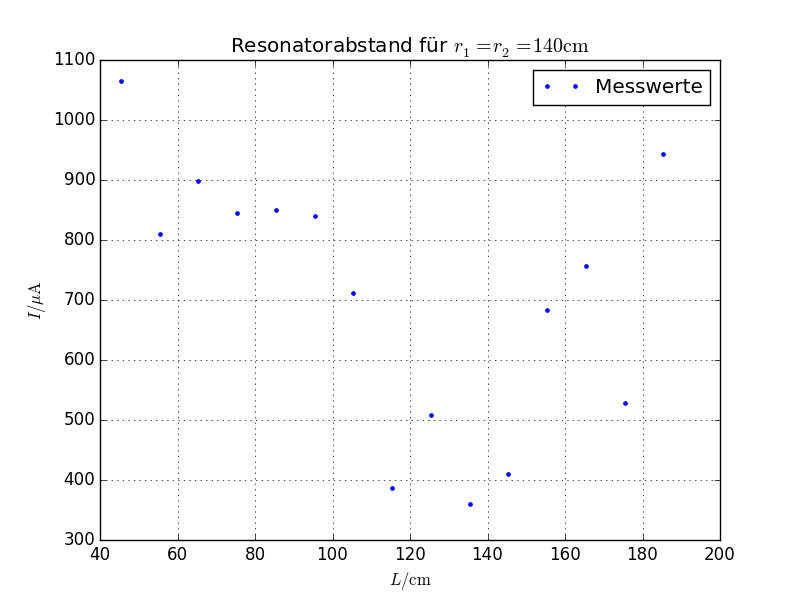
\includegraphics[width=0.5\textwidth]{plots/stabil1}
	\caption{Resonatorlänge gegen Strom bei gleich gekrümmten Spiegeln \(r_1=r_2=1,4\)m}
	\label{fig:stabil1}
\end{figure}

\noindent Für Spiegel mit den Krümmungsradien \(r_1\neq r_2\) ist die Nullstelle der Funktion bei \(L=r_1\lor L=r_2\). Die Funktion wird für \(L=r_1+r_2\) gleich eins.

\noindent Da bei der zweiten Spiegelkombination \(r_1=\infty\)m ist (planarer Spiegel), vereinfacht sich die Bedingung zu:

\begin{equation}
0\le1-\frac{1}{r_2}L<1
\end{equation}

\noindent was eine Geradengleichung mit negativer Steigung ist. Daraus folgt direkt, dass die Bedingung für das Intervall \(\mathbb{L}=(0,140]\). Die gemessenen Werte sind Tabelle \ref{tab:t2} zu entnehmen.

\begin{table}[H]
	\begin{center}
		\begin{tabular}{c c}
			\toprule
			\(L+L_0\)/cm & \(I\)/\(\mu\)A \\
			\midrule
			55              &272\\                                                                           
			65              &291\\                                                                             
			75              &120\\                                                                               
			85              &150\\                                                                                 
			95              &60\\                                                                                  
			105             &45\\
			\bottomrule
		\end{tabular}
		\caption{Resonatorlänge und Photostrom für \(r_1=\infty\)m, \(r_2=1,4\)m}
		\label{tab:t2}
	\end{center}
\end{table}

\noindent Die graphische Darstellung von \(L\) gegen \(I\) ist in Abbildung \ref{fig:stabil2} gegeben.

\begin{figure}
	\centering
		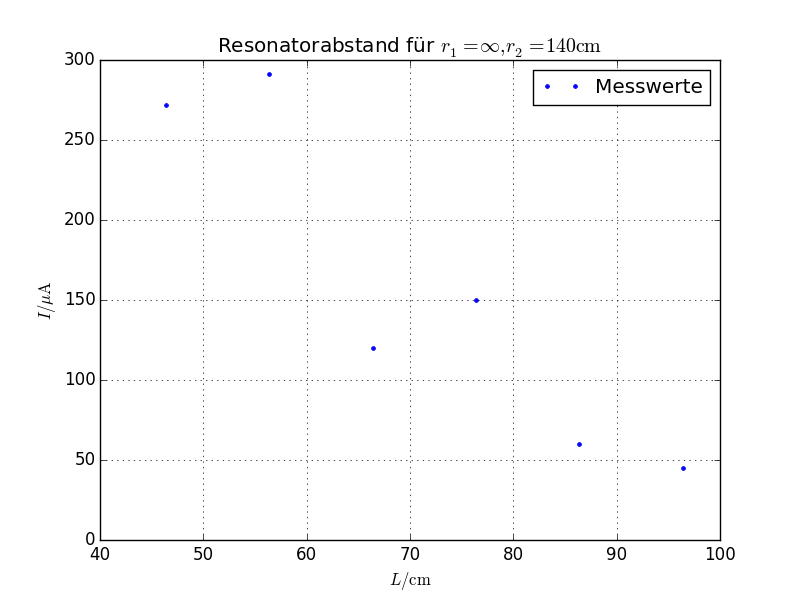
\includegraphics[width=0.5\textwidth]{plots/stabil2}
	\caption{Strom gegen Resonatorlänge mit planarem Spiegel \(r_1=\infty\)m, \(r_2=1,4\)m}
	\label{fig:stabil2}
\end{figure}

\subsection{TEM-Moden}
Die Intensitätsverteilung der Grundmode wird durch Formel \ref{eq:gauß} beschrieben. Dabei ist \(d\) der Abstand zur optischen Achse und \(w\) der Strahlendurchmesser. Die theoretische Kurve wird durch nichtlineare Ausgleichsrechnung and die Messwerte angepasst. Für die Parameter ergibt sich dann:


\begin{equation*}
I_0=6,17\pm0,12
\end{equation*}

\begin{equation*}
d_0=-3,79\pm0,12
\end{equation*}

\begin{equation*}
w=10,58\pm0,24
\end{equation*}

\noindent Die Messwerte und die Ausgleichskurve sind in Abbildung \ref{fig:TEM00} dargestellt. Die Messwerte sind Tabelle \ref{tab:t5} zu entnehmen.

\begin{figure}
	\centering
	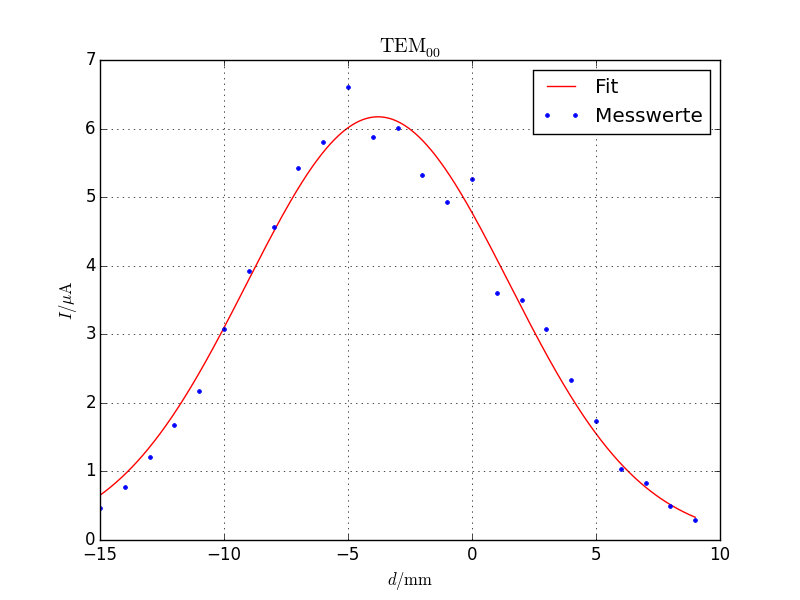
\includegraphics[width=0.5\textwidth]{plots/TEM00}
	\caption{Messung der TEM\(_{00}\)-Mode}
	\label{fig:TEM00}
\end{figure}

\begin{table}[H]
	\begin{center}
		\begin{tabular}{c c}
			\toprule
			\(d\)/mm & \(I\)/\(\mu\)A \\
			\midrule
			-15  &  0,46\\                                                                                            
			-14     &0,77\\                                                                                          
			-13     &1,21\\                                                                                        
			-12     &1,68\\                                                                                      
			-11     &2,17\\                                                                                    
			-10     &3,08\\                                                                                  
			-9      &3,93\\                                                                               
			-8      &4,56\\                                                                             
			-7      &5,42\\
			-6      &5,80\\                                                                         
			-5      &6,61\\                                                                       
			-4      &5,88\\                                                                     
			-3      &6,01\\                                                                   
			-2      &5,33\\
			-1      &4,93\\
			0       &5,27\\
			1       &3,60\\
			2       &3,50\\
			3       &3,08\\
			4       &2,33\\
			5       &1,73\\
			6       &1,04\\
			7       &0,83\\
			8       &0,50\\
			9       &0,29\\
			\bottomrule
		\end{tabular}
		\caption{Position der Photodiode bei transversaler Verschiebung und zugehörigem Photostrom}
		\label{tab:t5}
	\end{center}
\end{table}

\noindent Die theoretische Intensitätsverteilung für die TEM\(_{10}\)-Mode ist:

\begin{equation}
I_{10}(d)=I_0(d-d_0)^2\cdot e^{-2\left(\frac{d-d_1}{w}\right)^2}
\end{equation}

\noindent Die Parameter ergeben sich aus der nichtlinearen Ausgleichsrechnung.

\begin{equation*}
I_0=(0,028\pm0,002)
\end{equation*}

\begin{equation*}
w=(10,052\pm0,235)
\end{equation*}

\begin{equation*}
d_0=(-2,480\pm0,186)
\end{equation*}

\begin{equation*}
d_1=(-3,49\pm0,18)
\end{equation*}

\noindent Die Messwerte und die Ausgleichskurve sind in Abbildung \ref{fig:TEM10} dargestellt. 

\begin{figure}[H]
	\centering
	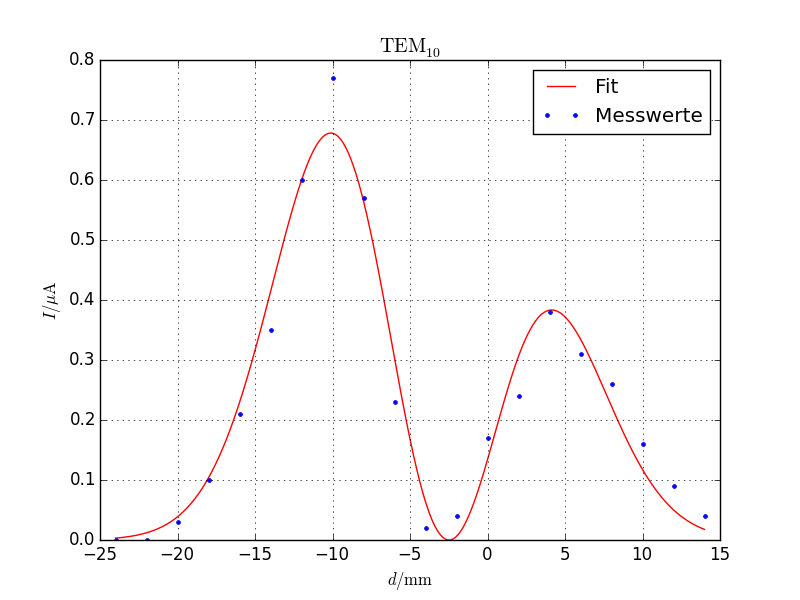
\includegraphics[width=0.5\textwidth]{plots/TEM10}
	\caption{Messung TEM\(_{10}\)-Mode}
	\label{fig:TEM10}
\end{figure}

\noindent Die Messwerte sind Tabelle \ref{tab:t6} zu entnehmen.

\begin{table}[H]
	\begin{center}
		\begin{tabular}{c c}
			\toprule
			\(d\)/mm & \(I\)/\(\mu\)A \\
			\midrule
			-24     &0\\
			-22     &0\\
			-20     &0,03\\
			-18     &0,10\\
			-16     &0,21\\
			-14     &0,35\\
			-12     &0,60\\
			-10     &0,77\\
			-8      &0,57\\
			-6      &0,23\\
			-4      &0,02\\
			-2      &0,04\\
			0       &0,17\\
			2       &0,24\\
			4       &0,38\\
			6       &0,31\\
			8       &0,26\\
			10     & 0,16\\
			12      &0,09\\
			14      &0,04\\
			\bottomrule
		\end{tabular}
		\caption{Position der Photodiode bei transversaler Verschiebung und zugehörigem Photostrom}
		\label{tab:t6}
	\end{center}
\end{table}

\subsection{Polarisation}
Die gemessenen Werte werden in einem Diagramm aufgetragen und durch die theoretische Kurve angepasst. Diese hat folgende Gestalt:

\begin{equation}
I=I_0\sin^2{(\phi-\phi_0)}\quad.
\end{equation}

\noindent Die nichtlineare Ausgleichsrechnung ergibt für die Parameter:

\begin{equation*}
I_0=453,37\pm8,31
\end{equation*}

\begin{equation*}
\phi_0=-88,24\pm0,02
\end{equation*}

\noindent Die graphische Darstellung der Messwerte und der Ausgleichskurve sind Abbildung \ref{fig:pol} zu entnehmen.

\begin{figure}[H]
	\centering
	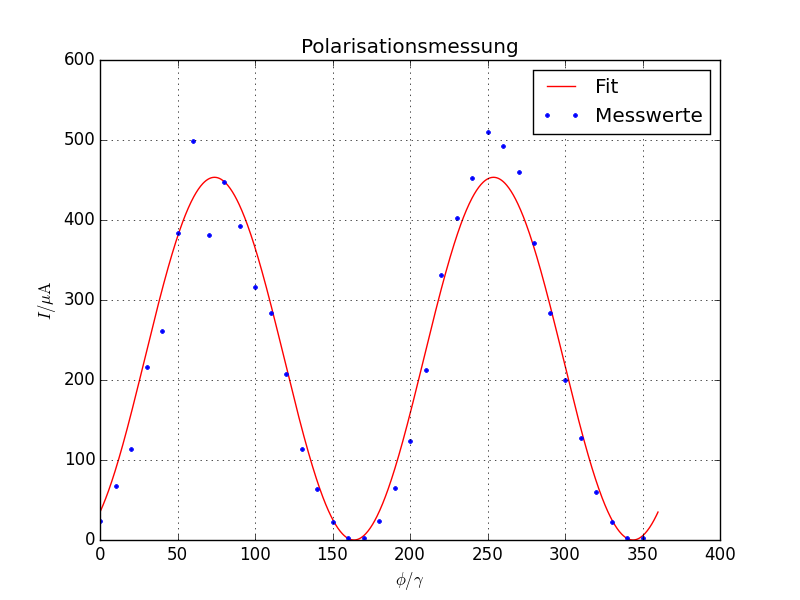
\includegraphics[width=0.5\textwidth]{plots/pol}
	\caption{Messung der Polarisation}
	\label{fig:pol}
\end{figure}

\noindent Die Messwerte sind Tabelle \ref{tab:t4} zu entnehmen.

\begin{longtable}[H]{c c}
	%\begin{center}
		%\begin{tabular}{c c}
			\toprule
			\(\phi\)/° & \(I\)/\(\mu\)A \\
			\midrule
			0       &24\\
			10      &67\\
			20      &114\\
			30      &216\\
			40      &261\\
			50      &384\\
			60      &499\\
			70      &381\\
			80      &448\\
			90      &393\\
			100     &316\\
			110     &284\\
			120     &207\\
			130     &114\\
			140     &64\\
			150     &22\\
			160     &2\\
			170     &3\\
			180     &24\\
			190     &65\\
			200     &124\\
			210     &213\\
			220     &331\\
			230     &403\\
			240     &453\\
			250     &510\\
			260     &493\\
			270     &460\\
			280     &371\\
			290     &284\\
			300     &200\\
			310     &127\\
			320     &60\\
			330     &23\\                                                                                            
			340     &2\\                                                                                         
			350     &3\\
			\bottomrule
		%\end{tabular}
		\caption{Photostrom für verschiedene Winkel des Polfilters}
		\label{tab:t4}
	%\end{center}
\end{longtable}

\subsection{Wellenlänge}
Die Gitterkonstante des Gitters beträgt \(g=\frac{1}{80}\cdot10^{-3}\text{m}\), der Abstand von der Quelle zum Schirm beträgt \(s=2\text{m}\). Es wurde, um den Fehler zu minimieren, der Abstand \(d\) von Maximum zu Maximum gemessen und das bis zur dritten Ordnung. Die Wellenlänge berechnet sich aus:

\begin{equation}
\lambda=\frac{g\cdot\sin{\left(\arctan{\left(\frac{d}{2s}\right)}\right)}}{n}\quad.
\end{equation}

\noindent Die gemessenen und berechneten Werte sind der Tabelle \ref{tab:t3} zu entnehmen.

\begin{table}[H]
	\begin{center}
		\begin{tabular}{c c c}
			\toprule
			Ordnung & \(d/\)m & \(\lambda/\)nm \\
			\midrule
			1 & 20 & 624,2\\
			2 & 40 & 621,8\\
			3 & 61 & 628,2\\
			\bottomrule
		\end{tabular}
		\caption{Messwerte des Interferenzmusters}
		\label{tab:t3}
	\end{center}
\end{table}

\noindent Die Wellenlänge ergibt sich daraus zu

\begin{equation*}
\lambda=(624,8\pm1,8)\text{nm}.
\end{equation*}